\chapter{Scrambling}\label{ch:Scrambling}
Security is not only about cryptography. But there is a main reason why 
cryptography is attacked, and that is because there is a very low 
chance of being detected. There will be no traces of the attack, since 
the attacker’s access will look just like an ordinary access.

This can be compared to a real-life break-in. The break-in will be 
noticed if the thief breaks in using a crowbar. On the other hand, you 
might never notice that the security had been breached, if the the 
thief were to pick the lock instead. \citep{Schneier:2003}

One of the more noteworthy cryptography rule is that you always are to 
assume that someone is out to get you. Because of this, 
\citet[pp. 12--14]{Schneier:2003} says that we always need to look for 
possible ways to break systems, to ensure that the security can not be 
breached, and thereby provides security.

\section{Why do we need cryptography?}
Cryptography is the science of rendering plaintexts into ciphertexts to 
protect contents from unauthorized viewing. It is used in electronic 
communication for protection of e-mail messages and credit card 
information among other things. If we send data without encrypting it, 
someone who is eavesdropping to the transmission channel will most 
likely access the data.

For most people this is not a problem, but in some instances sending 
secure messages can be extremely important. One example is 
communication during war, where a single piece of intelligence might 
turn the tide of the entire war. You might also not want people to be 
able to read your account information and card numbers when buying 
things online either.

\Warning[Source]{Typ Schneier har jag för mig? Låna om boken?}
%This might need a rework!

Another reason for scrambling is to reduce the number of adjacent 
data bits with the same value, like strings of zeroes or ones. It could 
also serve to balance the number of zeroes and ones in strings. This is 
done as to try to obtain DC balance. DC balance is desired since it 
avoids voltage imbalance during communication between connected systems.

\Warning[Rewrite]{And find a good source for this}
%Det är osannolikt att det här stämmer helt och hållet :)

\section{Scrambling or Encrypting}
Scrambling can be seen as the distortion of a plain-text, using a CW. 
Encryption can, on the other hand, be seen as the entire process of 
protecting content, from generating the CW to scrambling the data. 
Scrambling can therefore be seen as a subset of encryption.

\section{Data packets}\label{sec:Data}
The data processed by the DVB systems is sent in data packets. All of 
them are created from Elementary Stream packets (ES) which are 
generally the output from an audio or video encoder. The ES-packets are 
then packeted into Program Stream- (PS), Transport Stream- (TS) or 
Packatized Elementary Stream (PES) packets and then distributed. Among 
the three ways of packing data, only two are interresting from a DVB 
perspective. This is due to PS packets being used for storing data, 
while TS and PES are used for transmitting data. The interresting 
types, when working with DVB, are therefore the TS packets as well as 
the PES packets. PES packets are often packed into the payload of TS 
packets.

\subsection{TS packets}
TS packets are the ones used by the DVB society, possibly due to their 
fixed lenghts. TS packets have got a length of 188 bytes with a 4 byte 
long header. This means that the payload consists of 184 bytes. The 
layout of a TS packet can be viewed in figure 
\ref{img:Package}\citep{DVB:2013}.

\begin{figure}
  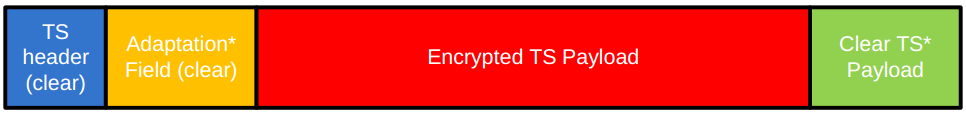
\includegraphics[width=\textwidth]{TSpacket}
  \caption{General layout of a data packet}
  \label{img:Package}
\end{figure}

The TS packet consists of 4 different kinds of building blocks where 
only the header is guaranteed to be present. Those blocks are:

\begin{itemize}
\item Header
\item Adaptation field
\item Encrypted payload
\item Clear payload
\end{itemize}

The byte-sizes of the building blocks are:

\begin{itemize}
\item header\_size = 4
\item adaptation\_field\_size = the size of the adaptation field
\item payload\_size = 188 - (header\_size + adaptation\_field\_size)
\item encrypted\_payload\_size = payload\_size - [payload\_size mod block\_size]
\item clear\_payload\_size = [payload\_size mod block\_size] 
  (or simply payload\_size - encrypted\_payload\_size)
\end{itemize}

\subsubsection{Header}
The header consists of information regarding the packet, 
and has a sync\_byte (with a hex-value of 0x47, or bit-value of 
01000111) to announce the beginning of a packet. The header also 
contains information as to whether there is an adaptation field and 
payload in the packet, what PID the packet has, if it is to be 
prioritized, whether the data is scrambled - and in that case if it 
was scrambled with an odd or even key, among others 
\citep[pp. 25--26]{etsiMPEG:2009}. The header is never to be encrypted 
and is always found at the beginning of a packet 
\citep[pp. 10--11]{DVB:2013}.

The header contains the following:
\begin{longtable}{l l l}
  Bits & Name & Description \\
  8 & Sync byte & Fixed byte value 0x47 \\
  1 & Transport Error Indicator & Uncorrectable bit errors exist. \\
  1 & Payload Unit Start Indicator & TS packet contains PES packets or\\
  & & Program Specific Information (PSI data)\\
  2 & Transport Scrambling Control & 00 No scramling, 01 Reserved, \\
  & & 10 Even key, 11 Odd key \\
  1 & Transport Priority & 1 gives this packet higher priority \\
  13 & PID & Type and number of data \\
  & & stored in packet payload \\
  1 & Adaptation Field Control & 1 means that an adaptation field exists\\
    1 & Contains Payload & 1 means that payload exists \\
    4 & Continuity Counter & Sequence number of payload packets\\
\end{longtable}

\subsubsection{Adaptation field}
The adaptation field is a sort of padding that is input when the end of 
the data does not align with the end of the TS packet. This is done to 
make sure that the TS packet is filled with known data. We only find 
adaptation fields when we are working with the last string of data, if 
the data does not align. Adaptation fields are not encrypted.
\cite[pp. 10--11]{DVB:2013}

\subsubsection{Encrypted and clear payload}
When working with block ciphers, we tend to end up with clear bytes of 
data since block ciphers only encrypt data blocks of fixed sizes. The 
clear data is always located at the end of the TS packets and might be 
of sizes up to one byte smaller than the block size (15 bytes for 
AES-128) at the most. The encrypted payload is always located in front 
of the clear payload. \cite[pp. 10--11]{DVB:2013}

\subsection{PES packets}
The PES packets have varying lengths of up to 64 kilo bytes, and are 
often packed into TS packets when distributed, due to the strength of 
TS packets. The payload data in the TS packets, when carrying PES 
packets, consist of the entire PES packets, which is the header as well 
as the data. PES packets do not use adaptation fields, since they are 
of adaptable lengths, as long as the length of the packet does not 
exceed 64 KBytes.

Since DVB seldom uses itself of PES packets, an analyzation of the 
header will not be done. The derivation of PES packets from TS packets 
can be seen in Figure \ref{img:PES} \citep[p. 9]{ETR:289}.

\begin{figure}
  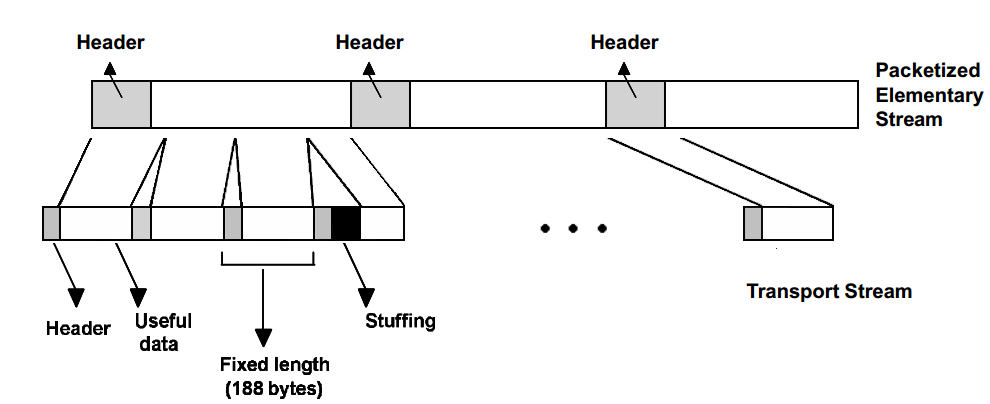
\includegraphics[width=\textwidth]{PES.png}
  \caption{PES packet derived from TS packets}
  \label{img:PES}
\end{figure}

\section{Encryption and Decryption}
There are two things that you need when you encrypt and decrypt 
messages. Those are the algorithm, plaintext and the key. Even though 
there are plenty of ways to encrypt messages, there are mainly two ways 
of sharing the encryption-key. The first method is the symmetric-key 
encryption, and the second method is the public-key encryption.

\subsection{Symmetric-key encryption}\label{ch:symmetric}
The symmetric-key encryption uses the same key to encode and decode 
messages. Distrubution of the key, when using the symmetric-key 
encryption is troublesome and the fact that both parties need access to 
the same secret key is a major drawback of the symmetric key 
encryption, as compared to the public-key encryption method. Sending 
the key in an email is a bad idea, since the persons who wants to read 
our messages most likely already will be listening, and they will 
therefore obtain the key as well as the means to decode the messages we 
send. Both the CSA and the AES encryption methods are symmetric-key 
encryptions, using the same key for encryption and decryption.

\subsection{Public-key encryption}\label{ch:public}
The public-key encryption uses a public key that anyone can look up, 
and a secret key that only one person knows 
\citep[pp. 25--32]{Simmons:1992}. For instance say that the two 
persons, Bob and Alice, want to communicate. Bob produces a keypair 
\(P_{Bob}\) (Bob’s public key) and \(S_{Bob}\) (Bob’s secret key) and 
publishes \(P_{Bob}\) for anyone to see. When Alice wants to send Bob a 
message, she looks up Bob’s public key \(P_{Bob}\), which she then uses 
to encode her message. When she sends Bob the message, Bob decodes the 
message using his secret key \(S_{Bob}\) \citep{Schneier:2003}.

\subsection{Combination}
The big question now is why we would use anything other than the 
public-key encryption, since it seems secure and easy to manage. The 
reason is that the public-key encryption is not as effective as the 
symmetric-key encryption. It is common to use a combination of those 
two since an easy and effective way to encrypt messages is what we 
desire. To do this we use a symmetric-key algorithm to encode the 
plaintext into ciphertext, and then we use the public-key encryption to 
encode the symmeteric-key we used to encode the plaintext. The encoded 
key is then sent together with the ciphertext to the recipient, who 
uses the secret key to decode the symmetric key, which is then used 
to decipher the ciphertext to obtain the plaintext.

Decryption is often performed by reversing the encryption. You need to 
know the algorithm, preferably through a mathematical representation, 
to calculate how to obtain the plaintext from the ciphertext. A 
description of how this is done for the CBC-mode (described in 
\ref{sec:BlockCipher}) is described in \ref{sec:CBCcalc} in appendix 
\ref{app:examples}. We assume that we know the decryption algorithm 
here for simplicity. \Warning[Source]{feels like a given, but still}

\section{Ciphers}
A cipher is the same as an algorithm, that operates on either 
plaintexts or ciphertexts to perform encryption or decryption. Figure 
\ref{img:ciphers} describes how the different kinds of ciphers can be 
split into sub-groups. The first branch splits into Classical-, 
Rotor Machine- and Modern ciphers. Substitution and Transposition are 
still used in modern algorithms. The Modern ciphers are the Private 
key and Public key (descibed in chapter \ref{ch:symmetric} and 
\ref{ch:public}). The CSA algorithm uses both the stream- and block ciphers, while the AES algorithm only uses a block cipher.

\begin{figure}
  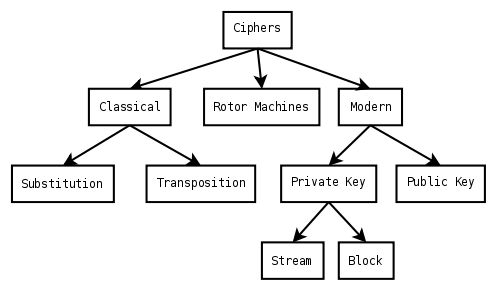
\includegraphics[width=\textwidth]{cipher.png}
  \caption{Different kinds of ciphers \citep{CipherTax:2013}}
  \label{img:ciphers}
\end{figure}

There are mainly two kinds of ciphers that are used when designing 
modern cryptosystems. Those ciphers are called block ciphers and 
stream ciphers. Many systems use a combination of block ciphers and 
stream ciphers to provide security. 

\Warning[Source]{At least the CSA uses it. But you need a source if you 
want this to be here}

\subsection{Block cipher}\label{sec:BlockCipher}
A block cipher operates on blocks where each block consists of a fixed 
number of bytes. This might cause a need for padding the blocks, in 
case the plaintext contains a number of bytes that is not even with the 
blocksize. Block cipher often use itself of a combination of S-boxes 
(Substitution boxes) and P-boxes (Permutation-boxes) in a so-called 
SP-network (Figure \ref{img:SPNetwork}).

There are many modes of block ciphers, but the two recommended by 
\citet{Schneier:2003} are the CBC-mode and the CTR-mode.

\emph{CBC} stands for \emph{cipher block chaining} and is performed by 
first encrypting the result of an XOR between an IV and the plaintext. 
This is the ciphertext that corresponds to the first plaintext. This is 
then put into an XOR with the next plaintext, and then encrypted 
\citep[pp. 109--111]{Stinson:2006}. For reference, see image 
\ref{img:CBCmode} in appendix \ref{app:fig}.

\emph{CTR} stands for \emph{counter}, and refers to the way the IV is 
generated. The counter outputs a value, which is encoded with the key. 
The output is then run in an XOR together with the plaintext, producing 
the ciphertext. The counter is then incremented and the procedure is 
iterated \citep[p. 111]{Stinson:2006}.

\subsection{Stream cipher} \label{sec:StreamCipher}
Stream ciphers work on a stream of data (as implied by the name). They 
usually consist of some kind of a keystream generator which performs a 
modulo 2 addition with the data \cite[pp. 67]{Simmons:1992}. An 
effective implementation of the stream cipher is to use a linear 
feedback shift-register which uses the current internal state (key) to 
produce the next state by a simple XOR-addition between two or more of 
the bits in the state. This is mainly used because of how easy it is to 
construct in hardware \citep{LFSR:2008}.

\section{Confusion and Diffusion}\label{ch:ConfDiff}
Two properties that are needed to ensure that a cipher provides 
security are confusion and diffusion \citep{Shannon:1949}. Note that a 
cipher is not secure just because these two properties are obtained.

\emph{Confusion} refers to making the relationship between ciphertext 
and key as complex as possible. \emph{Diffusion} refers to replacing 
and shuffling the data, to make it impossible to analyze data 
statistically. This is usually done by performing substitutions and 
permutations in a simple pattern multiple times. This can easily be 
done by using an SP-network (S-box / P-box network) 
\citep[pp. 74--79]{Stinson:2006}. The very first, as well as last step, 
of SP-Networks is usually an XOR between the subkey and the data. This 
is called \emph{whitening}, and is according to 
\citet[p. 75]{Stinson:2006} regarded as a very effective way to prevent 
encryption/decryption without a known key. The goal of this is to make 
it hard to find the key, even though one has access to multiple 
plaintext/ciphertext pairs produced with the same key 
\citep{Shannon:1949}.

\subsection{S-boxes}
The S-box is one of the basic components that is used when creating 
ciphers. An S-box takes a number of input bits and creates a number of 
output bits in a non-linear fashion \citep[pp. 74--75]{Stinson:2006}. 
They can effectively be implemented as lookup tables. Each input has to 
correspond to a unique output, to make sure that the input can be 
recreated in the descrambler.

% CONFUSION OR DIFFUSION?

\subsection{P-Boxes}
The second basic component used in cryptography is the P-box. A P-box 
shuffles / rearranges the order of given bits. This can be viewed in 
the SP-network in figure \ref{img:SPNetwork}, where the P-box is 
represented by the dotted rectangle in the middle.

\begin{figure}
  \begin{center}
    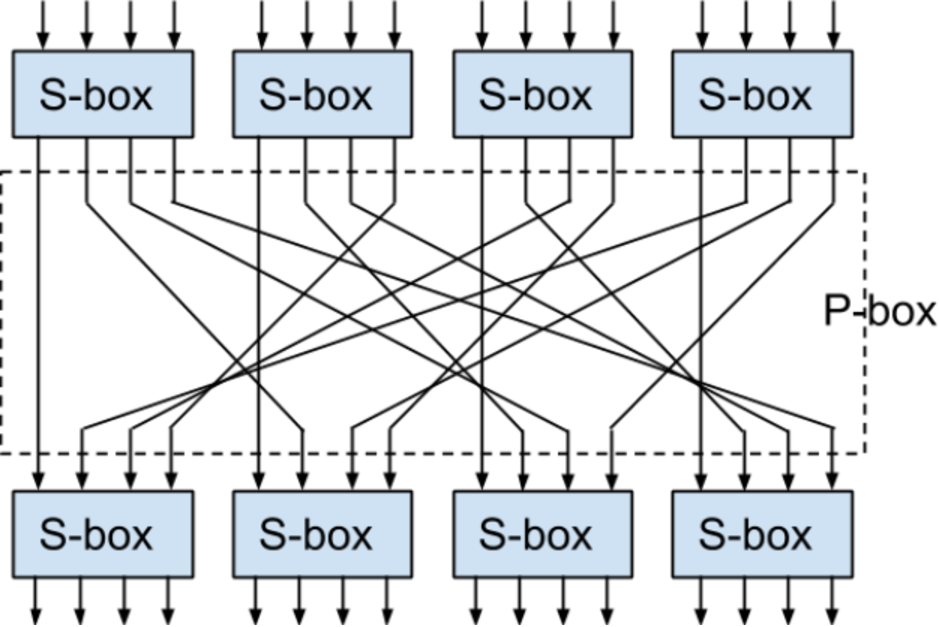
\includegraphics[width=0.5\textwidth]{SPnetwork}
    \caption{SP-Network}
    \label{img:SPNetwork}
  \end{center}
\end{figure}

%CONFUSION OR DIFFUSION?

\section{Secrecy}
Although encryption is important, as well as the strength of the 
encryption, keeping the algorithm secret is never a good idea. A simple 
mistake when designing an algorithm might turn an encryption that would 
otherwise have been strong, incredibly weak. It is therefore a bad 
idea to use small scale algorithms (designed for the use of just a few 
persons for instance). If you instead use an open algorithm, faults 
will most likely be discovered and fixed by experienced cryptographers 
\citep[pp. 23]{Schneier:2003}. Keeping the key, which is used to 
encrypt the data, secret is what is important.
